\textit{\textbf{AutoQuad} is the flight controller used in this project.
The author was among the first students using \ac{AQ} on \ac{SDU}, but the first student to make changes to the firmware and to communicate with \ac{AQ} over \ac{CAN}-bus.
The \ac{AQ} firmware was not very documented, so much time was spend reading through code and trying to figure out how it works.
A great amount of time was also spend on more practical things like getting to know their Development Environment (CrossWorks for ARM)\footnote{\url{http://www.rowley.co.uk/arm/} last visited 29 Maj} in order to compile their firmware, waiting for Quatos \footnote{The controller, Quatos, used in AQ is not Open Source so a license had to be acquired by SDU} license and getting familiar with the flashing process of the M4 board.
Much of the gained knowledge about \ac{AQ} and how to do debugging has been written down to share with other students.}
\footnote{It can be found in \textit{Appendix/SDU-UASAutoQuaddocumentation.pdf} \\ and \textit{SDU-UASAutoQuadsourcecodedocumentation.pdf} Text marked with green is written by the author} \\


Since \ac{AQ} only supports receiving absolute positioning through a serial port\footnote{Seen by inspection of the schematic to the M4-board done by the supervisor} another way had to be found.
The M4 board is born with an onboard ublox M8Q \footnote{\url{http://autoquad.org/wiki/wiki/m4-microcontroller/m4-gps-antenna-options/} last visited 29 Maj} which uses ublox's ubx protocol. If the M8Q GNSS was repleace everything sent by eg. a RPI has to be encoded as ubx.
The CAN-bus was chosen since it is already implemented and used in \ac{AQ}. \ac{AQ} supports sensor inputs through CAN, unfortunately GNSS was not supported and thereby had to be implemented.

\ac{AQ}s CAN protocol is described, implemented and tested in appendix \ref{app:aq_can_protocol}.
When the AQ M4 board boots, it tries to register the CAN nodes on the bus. The registering of CAN nodes has been described in appendix \ref{app:reg_aq_node}\\

When all CAN-nodes have successfully registered, different node-initializing functions is invoked.
First a summary run which sends the number and types of the nodes to QGroundStation. \footnote{Graphical userinterface which provides general information about the drone such as battery level, attitude but also waypoint functionality}.
It can thus be validated by the pilot that all the ESC's and CAN-sensors are detected.
After the summary the CAN-sensor initialization is invoked which creates a callback that gets attached to the CAN-type which in this case is CAN-sensor\footnote{CAN-types are described in section \ref{app:data_bits}}. When \ac{AQ} receives a sensor reading the callback will then be invoked nd the sensor value will be added to the array.\\

The callback default fills in the received sensor value in an array so the sensor value can be used in another task.
The canID \footnote{The canID is described in appendix \ref{app:data_bits}} is used as index so the task that needs the sensor value knows on which element in the array to look. Code \ref{code:callback} shows the default callback \footnote{\url{https://github.com/bn999/autoquad/blob/master/onboard/canSensors.c} last visited 29 Maj}
\begin{lstlisting}[language = c, caption = Callback invoked when a CAN-sensorvalue is received. It stores the value in an array indexed by canId. Note that the sensor value is casted to a float, label=code:callback]
void canSensorsReceiveTelem(uint8_t canId, uint8_t doc, void *data) {
    canSensorsData.values[canId] = *(float *)data;
	/* Reception time of the message stored as well */
}
\end{lstlisting}
The callback is fairly simple and does not save the doc\footnote{DOC is described in appendix \ref{app:data_bits}} which is needed in order to tell which message the CAN-GNSS sensor is sending. The messages received over CAN on the AQ M4 board is shown in section \ref{sec:system_indoor_drone}\\

All of the CAN-GNSS message handling has been implemented in the callback function. A more generic solution might have been to create a task and use a semaphore to signal when there is a new GNSS-packet available. Due to lack of time, everything was implemented in the callback.

Code \ref{code:psudo_parse_can_gps} shows a pseudo code of how the GNSS-messages is handled.

\begin{lstlisting}[language = Matlab, caption = Modified callback invoked when a sensor-value is received. Shows how DOC is used to tell which GNSS-message is received and when height is received the flags are set to update the \ac{UKF}, label=code:psudo_parse_can_gps]
canSensorsReceiveTelem(canId, doc, *data) {
	if doc == CAN_DOC_LAT then
		canData.latitude = data
		
	if doc == CAN_DOC_LON then
		canData.longitude = data
		
	if doc == CAN_DOC_DOP then
		canData.pDOP = data[0]/10
		..
	if doc == CAN_DOC_ACC then
		canData.satellites = data[0]
		canData.fix = data[1]
		canData.xAcc = data[x]/10
		..
		canData.heading = data[n-1]/100
		
	if doc == CAN_DOC_VEL then
		gpsData.velx = data[x]/100
		..		
	if doc == CAN_DOC_ALT then
		gpsDatat.height = data
		if gpsData.satellites >= 5 then
			gpsUpdatetime = now()
			setFlag (gpsData.gpsPosFlag)
			setFlag (gpsData.gpsVelFlag)
		else:
			debug_to_QGroundStation
}
\end{lstlisting}

The \textit{data} pointer given as parameter to the callback is of void pointer. Some pointer gymnastics is done in order to get the right elements from the CAN-packet. If the received CAN-packet is of 8*1 bytes, the void pointer is casted to an uint8\_t pointer so each byte can be retrieved by using the casted pointer as an array. 
2 bytes are allocated for each velocity, speed and heading. In order to send 2 decimals, each value was multiplied by 100 when sending and divided by 100 when received by \ac{AQ}.
Only one decimal for rest of the values was deemed necessary and was thereby multiplied and divided by 10.

When the flags are set, the task updating the \ac{UKF} will run \footnote{\url{https://github.com/bn999/autoquad/blob/master/onboard/run.c\#L110} last visited 23 maj}.
Code \ref{code:ukf_update} shows a snippet from the task updating the UKF when the position or velocity flag is set.
\begin{lstlisting}[language = Matlab, caption = Snippet of run.c as psudeocode which updates the UKF when position flag or velocity flag is set, label=code:ukf_update]
if IsFlagSet(gpsData.gpsPosFlag) == yes then
	    navUkfGpsPosUpdate(gpsData.lastPosUpdate, gpsData.lat, gpsData.lon, gpsData.height, ....);
	    ClearFlag(gpsData.gpsPosFlag);
	    
else if IsFlagSet(gpsData.gpsVelFlag) == yes then
	    navUkfGpsVelUpdate(gpsData.lastVelUpdate, gpsData.velN, gpsData.velE, ....);
	    ClearFlag(gpsData.gpsVelFlag);
\end{lstlisting}

Testing of the GNSS spoofing was done in cooperation with Kjeld Jensen since results was needed for the paper.
Before mounting an expensive RTK-GNSS on the drone, it was tested using a NEO-6P GPS. The tests can be seen in appendix \ref{app:test_of_spoofed_GNSS}
When testing was successful using the NEO-6P, the RTK-GNSS was mounted on the EduQuad.
Figure \ref{fig:rtk_test_route} shows the waypoints generated to test the performance of the RTK-GNSS and the tracked path.

\begin{figure}[H]
    \center
    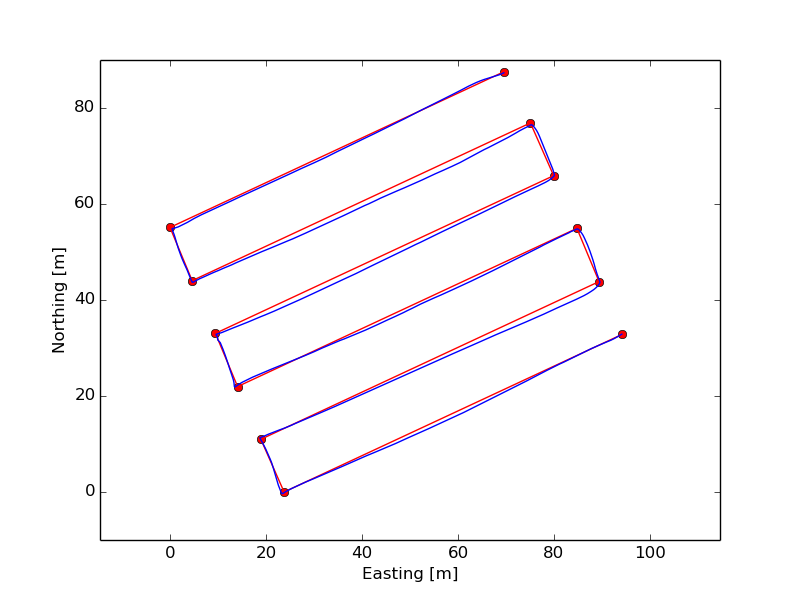
\includegraphics[width=0.7\textwidth]{graphics/rtk_test_planner.png}
    \caption{ Map of the planned route (red) with waypoints (red dots) and tracked flight (blue) }
    \label{fig:rtk_test_route}
\end{figure}
In figure \ref{fig:rtk_test_route} the dots represents waypoints, straight lines represents legs and the line deviating from the legs are the track of the drone.

Figure \ref{fig:rtk_test_route} shows the result of the test flight. 



\textit{The horizontal lateral distance is calculated as the distance to the closest point of any of the route legs.
This result in some inaccuracy at the end of each leg, and the hovering at the end of each leg skews the result slightly as well.
The measured average horizontal lateral distance from the route was 0.45 m.
The 95’th percentile was 1.11 m and the maximum distance was 1.35 m.
Figure \ref{fig:rtk_test_hist} shows a histogram of the horizontal lateral distances from the planned route.
The average vertical distance from the route was 0.26 m, the 95’th percentile was 0.72 m and the maximum distance was 1.52 m.} \footnote{Jensen, K.; Larsen, R.; Laursen M.S.; Neerup, M.M.; Skriver, M. and Jørgensen, R.N. Towards UAV contour flight over agricultural fields using RTK-GNSS and a Digital Height Model}

The reason for the relatively low accuracy of flying with the RTK-GNSS is out of the scope of this project.

\begin{figure}[H]
    \center
    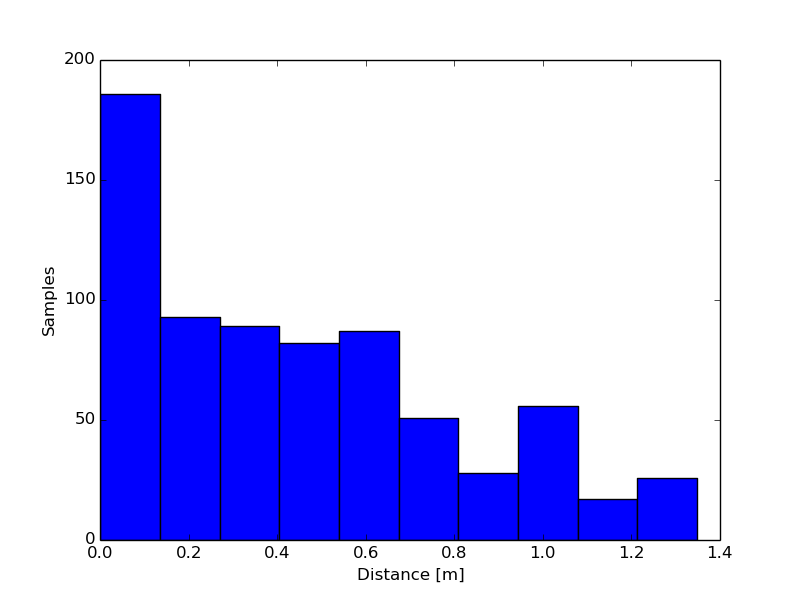
\includegraphics[width=0.7\textwidth]{graphics/rtk_test_hist_dist.png}
    \caption{Histogram of the horizontal lateral distance from the drone to the planned
route during the experiment. The total number of GPS track points (samples) is 715.}
    \label{fig:rtk_test_hist}
\end{figure}

It can be concluded that it is possible to inject absolute GNSS positions into the \ac{AQ} M4 board over \ac{CAN}. The tests made in appendix \ref{app:test_of_spoofed_GNSS} shows it is possible to decide how much the UKF should trust the GNSS positions based on the DOP values.